%%%%%%%%%%%%%%%%%%%%%%%%%%%%%%%%%%%%%%%%%%%%%%%%%%%%%%%%%%%%%%%%%%%%%%%%

%% \CharacterTable
%%  {Upper-case    \A\B\C\D\E\F\G\H\I\J\K\L\M\N\O\P\Q\R\S\T\U\V\W\X\Y\Z
%%   Lower-case    \a\b\c\d\e\f\g\h\i\j\k\l\m\n\o\p\q\r\s\t\u\v\w\x\y\z
%%   Digits        \0\1\2\3\4\5\6\7\8\9
%%   Exclamation   \!     Double quote  \"     Hash (number) \#
%%   Dollar        \$     Percent       \%     Ampersand     \&
%%   Acute accent  \'     Left paren    \(     Right paren   \)
%%   Asterisk      \*     Plus          \+     Comma         \,
%%   Minus         \-     Point         \.     Solidus       \/
%%   Colon         \:     Semicolon     \;     Less than     \<
%%   Equals        \=     Greater than  \>     Question mark \?
%%   Commercial at \@     Left bracket  \[     Backslash     \\
%%   Right bracket \]     Circumflex    \^     Underscore    \_
%%   Grave accent  \`     Left brace    \{     Vertical bar  \|
%%   Right brace   \}     Tilde         \~}

%%%%%%%%%%%%%%%%%%%%%%%%%%%%%%%%%%%%%%%%%%%%%%%%%%%%%%%%%%%%%%%%%%%%%%%

%\documentclass[b5paper,10pt,twoside,cucitura]{toptesi}
\documentclass[b5paper,10pt]{toptesi}

%%%PACKAGES%%%

\usepackage{lipsum}
\usepackage{amssymb} %per i simboli degli insiemi numerici
\usepackage{amsthm} %per \proof e \endproof
\usepackage{ragged2e} %giustifica
\justifying %giustifica
\usepackage{eurosym}
\usepackage{graphicx}
\usepackage{empheq}
\usepackage{xcolor}
\usepackage{amsmath}
\usepackage[T1]{fontenc}
\usepackage[latin1]{inputenc}
\usepackage{lmodern}
\usepackage{hyperref}
\usepackage[titletoc,toc,title]{appendix}

\hypersetup{%
    pdfpagemode={UseOutlines},
    bookmarksopen,
    pdfstartview={FitH},
    colorlinks,
    linkcolor={blue},
    citecolor={red},
    urlcolor={blue}
  }

%%%FRONTISPIECE%%%

\ateneo{Universit{\`a} degli Studi di Milano-Bicocca}
\FacoltaDi{Statistica\\e Metodi Quantitativi per la finanza}
\titolo{Improving Overnight Curve Calibration}
\corsodilaurea{Economia e Finanza}
\candidato{\tabular{@{}l@{}}Nicholas \textsc{Bertocchi}\\matricola: 797940\endtabular}
\relatore{prof.\ Ferdinando Ametrano}
%\secondorelatore{prof.\ .....}
\tutoreaziendale{dott.\ Nicola Moreni}
\NomeTutoreAziendale{Banca IMI}
\sedutadilaurea{\textsc{Anno~accademico} 2015-2016}
\logosede{logo}

\newtheorem{osservazione}{Osservazione} %Standard LaTeX
\begin{document}\errorcontextlines=9 %debugging
\english
\CycleName{cycle}

	\CorsoDiLaureaIn{Master degree course in\space}
	\NomeMonografia{Bachelor Degree Thesis}
	\TesiDiLaurea{Master Degree Thesis}
	\InName{in}
	\CandidateName{Candidate}% or Candidate
	\AdvisorName{Supervisors}% or Supervisor
	\TutorName{Tutor}
	\NomeTutoreAziendale{Internship Tutor:\\Banca IMI}
    \CycleName{cycle}

\frontespizio

%\ringraziamenti

\indici
\mainmatter

%%%ABSTRACT%%%

%\chapter*{Abstract}
%\markboth{\MakeUppercase{Abstract}}{}
%\addcontentsline{toc}{chapter}{Abstract}

%%%INTRODUCTION%%%

\chapter*{Introduction} \label{chap:Intro}
\markboth{\MakeUppercase{Introduction}}{}
\addcontentsline{toc}{chapter}{Introduction}
Every work which seeks to speak about interest rates term structure cannot avoid to begin from 2007 liquidity and credit crisis. Before that harmful year every market participants considered the credit risk on short time frame, for example less then one year, irrelevant and this opinion was reflected by the market in infinitesimal basis spread between different tenor rates. In other words, all banks in the system consider almost the same lend money to other banks for a year, for a month or for a day and this was possible because a big financial institution's default probability was seen as negligible. Otherwise it wasn't, as the Lehman Brothers case teach to the world. The panic in the markets during summer 2007 drives first to a crisis of confidence between the so called "Too big to fail" \footnote{This title was created during subprime crisis to speak about financial institutions that, as the nickname suggest, are so big that their default might means the overall system collapse} that, unable to estimate other institutions creditworthiness, can't no more trust each other and this leads to a situation in which it was preferable to be paid with higher frequency in order to mitigate counterparts credit risk. The direct consequence was that Libor as well as Euribor rates with different tenors shown different portions of credit/liquidity spread which became higher as tenor increase. That was the end of the Single-Curve World. From that time every implied relationship between interest rates failed and it become necessary to calibrate, for each currency, multiple forwarding curve and particular relevance was given to the Overnight Curve (from now ON) which plays the role of forwarding curve for its specific tenor and the role of exogenous discounting curve for each tenor. This double function is due to the fact that all interest rate derivatives traded on regulated markets (like Futures) or collateralized with daily margining (like Forward Rate Agreements, Swaps and Basis Swaps) settle their positions on collateral accounts which earn the overnight rate and this is why the ON Curve usually plays the role of discounting curve as well as the role of forwarding curve.\\
This work aims to discuss how a "state of art" ON curve can be calibrated starting from some general rate curve bootstrapping issues, presented in Chapter ..., like:

\begin{description}
    \item{-} Curve parametrization;
    \item{-} Bootstrap Algorithms;
    \item{-} Pillar interpolation technique.
\end{description}

After that, Chapter ... will be focused on the ON curve construction explaining which kind of choice are preferable passing through the same points outlined in Chapter ....
Finally, Chapter ... represents the core of this work and analyze some peculiar overnight problems outlining different solutions in order to improve the ON curve quality. In particular this point will be stressed:

\begin{description}
    \item{-} Forward Stub utilization to prevent Overlapping instruments;
    \item{-} Jumps and Turn of Year \textit{(TOY)} effect fixing in foreign currencies curve (the GBP and USD problem will be presented);
    \item{-} Fed Funds Arithmetic Average Coupon OIS introduction to Increase USD curve smoothness.
\end{description}

%%%CHAPTER1%%%

\chapter{Rate Curve Bootstrap} \label{chap:1}
    \section{Parametrization} \label{section:1.1}
        \subsection{Description through Forward Rates} \label{subsection:1.1.1}
        \subsection{Classical solution through Discount Factors} \label{subsection:1.1.2}
    \section{Calibration Algorithms} \label{section:1.2}
    Pricing of all interest rate derivatives requires modelling the future dynamics of the zero rates (or yield) curve term structure. A key point to understand is that finding the best way to build the rates term structure is crucial in order to obtain reasonable price, since an incorrect one will fail to produce them. The aim to which we have to be targeted on when calibrating an yield curve is to minimize, or eliminated, repricing errors especially on the most liquid instruments that are the one preferred for calibration as it will be discussed in .... 
    In order to fulfil our task of error minimization there are different ways that can be divided into 2 main classes that, as a common condition, both require a set of $N$ pre-selected market instruments:
    \begin{itemize}
        \item Best-Fit Algorithm
        \item Exact-Fit Algorithm
    \end{itemize}
        \subsection{Best Fit Algorithm} \label{subsection:1.2.1}
        A {\it best-fit algorithm} assumes a functional form for the curve $\{C_{x}\}$ and calibrates its parameters using the pre-selected instruments. It is very popular due to the smoothness of the output curve, calibration easiness and intuitive financial interpretation but it has a big drawback: usually there are more instruments than parameters and this lead to a relevant problem consisting in an imperfect reprice of the whole set of instruments. The merely fact that a best-fit calibration minimize instead of eliminate repricing errors means that this kind of algorithm are not good enough for trading purposes in liquid markets, where the market's deepness and the Bid/Ask spread closeness implies that a basis point quarter can make the difference.
        \subsection{Exact Fit Algorithm} \label{subsection:1.2.2}
        {\it Exact-fit algorithms}, instead, fix the yield curve on a time grid of $N$ points (or {\it pillars}) in order to exactly reprice the selected instruments. To do that, An interpolation method is required to determine curve values between pillars. Usually the algorithm is incremental, building the curve step-by-step with the increasing maturity of the ordered instruments ({\it bootstrap} approach).\\
        The set of bootstrapping instruments defines the time grid used for bootstrapping: each pillar is the maturity date or the last relevant date of the corresponding instrument.
        The interpolation method is strictly connected to the bootstrap and plays a fundamental role also during bootstrapping and not just after that. The "pillar-to-pillar" calibration proceeds with incomplete information; so, in order to determine each pillar value, the already bootstrapped part of the curve has to be used and, in particular, both pillar and intermediate interpolated values. This is the reason why we need to interpolate during the bootstrap algorithm and it also explain why this process is iterative. In fact, if the algorithm determines next pillar value taking advantage of the pre-bootstrapped part of the curve, it is straightforward that this value is influenced by it. Since including a pillar means add new information concerning the curve dynamic, if we use a {\it global interpolation scheme}, this tends to alter the first curve part shape (as it will be discussed in ....). This is usually remedied by cycling in iterative fashion: after a first bootstrap the resulting complete grid is altered one pillar at time using again the same bootstrapping algorithm, until convergence is reached (see "haganwest" for a practical example of this interaction between interpolation and bootstrap).\\
        Clearly, this kind of algorithms are more accurate; henceforward we restrict the analysis to the exact curve calibration problem.
    \section{Interpolation Techniques} \label{subsection:1.3}
    Whatever parametrization and algorithm has been chosen, an interpolation for off-grid dates/times is needed. An interpolation technique always work with two distinct objects:
    \begin{description}
        \item{-} the quantity to be interpolated;
        \item{-} the interpolation scheme.
    \end{description}
    The quantity to be interpolated is chosen according to curve's description. If we use a description through forward rates, the most reasonable quantity to be interpolated is the forward rate itself: in this way interpolation schemes and constraints can be imposed directly on market quantities. If we have to use a description through pseudo-discount factors (and this is our case as discuss in ....) we have the following main choices: discount factors, zero rates, instantaneous forward rates. In particular discount factors have exponential decay; so it makes sense to interpolate on log-discounts. Before analyzing the different impact of different choices on curve smoothness we have to introduce the interpolation scheme concept. 
        \subsection{Local scheme Vs. Global scheme} \label{subsection:1.3.1}
        We can group all interpolation techniques into 2 different classes:\\
        \begin{itemize}
        \item{\bfseries Local scheme}: each intermediate point depends only on its bracketing pillars. Notice that when bootstrapping with a local interpolation the curve's shape between two calibrated pillars can no longer change. This kind of scheme use only $\{y\ped{i}\}$ near $\{t\ped{i}\}$ to calculate each $\{y'\ped{i}\}$ and a typical example is the linear interpolation.
        \item{\bfseries Global scheme}: each intermediate point depends on points outside the interval defined by its neighborhoods pillars. If the interpolation method is global, the curve changes continuously until the end of the procedure because the shape of the part of the curve already bootstrapped is altered by the addition of further pillars as stressed in ..... Cubic spline are the most common examples of global interpolations that are fully defined when function values $\{y\ped{i}\}$ at point $\{t\ped{i}\}$ are supplemented with function first derivatives values $\{y'\ped{i}\}$.\\
        \end{itemize}
        
        \begin{figure}[!h]
        \centering
        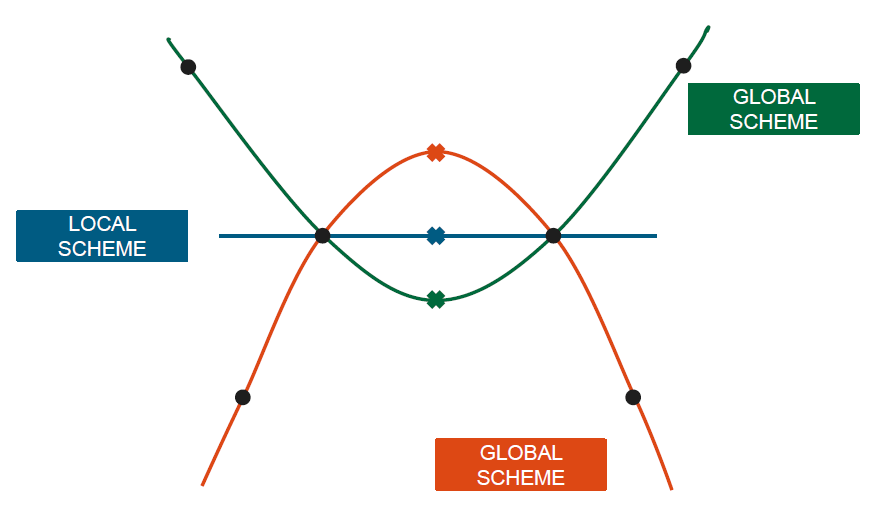
\includegraphics[width=0.8\textwidth]{images/scheme.PNG}
        \caption{Local scheme Vs. Global scheme interpolation.}
        \label{fig:scheme}
        \end{figure}
        
        \newpage
        The criteria used to analyse the interpolation techniques usually fall into one of the following two categories:
        \begin{itemize}
        \item the quality of the forward rates: in this case we are looking at the curve as an "accounting" tool and we are trying to answer the question "How good the forward rates look?"; 
        \item the quality of the implied hedging strategies: in this case we are looking at the curve as a "risk management" tool and we are trying to answer the question "Are the implied hedging quantities reasonable and stable?"
        \end{itemize}
        Sometimes an interpolation method is good to build forward rates but not good from an hedging point of view (This is the case of cubic spline). Since we are not interested to discuss the implementation of hedging curve we will restrict our analysis focusing on the object of building high quality forward rates.
        We now menage all requirements to introduce and discuss some of the most popular interpolation techniques (i.e. quantity to be interpolated plus an interpolation scheme) stressing on every pros and cons.\\
        Since each simple forward rate is approximately the integral of instantaneous forward rates, we will analyze the smoothness of simple forward rates computing instantaneous forward rates. The starting point is a set of known curve's points $\left\{ (t_{i},y_{i}=y(t_{i}))\right\}_{i=1,...,N}$ where $y$ represent the quantity to be interpolated as defined above. $t_{0}$ will be the reference date.
        \subsection{Linear and Log-Linear interpolation} \label{subsection:1.3.2}
        This is a poor and simple way to interpolation that can be computed directly on zero rates (Linear) or on log-discounts (log-linear). For $t \in [t_{i-1}, t_{i}]$ the piecewise linear interpolation formula for zero rates is: $$z(t)t=\frac{t-t_{i-1}}{t_{i}-t_{i-1}}z(t_{i})t+\frac{t_{i}-t}{t_{i}-t_{i-1}}z(t_{i-1})t$$
        This kind of interpolation techniques produces the so called: "Sawtooth forward rates" as visible in Figure \ref{fig:piecewiselinear} and Figure \ref{fig:sawtooth}:
        
        \begin{figure}[!h]
        \centering
        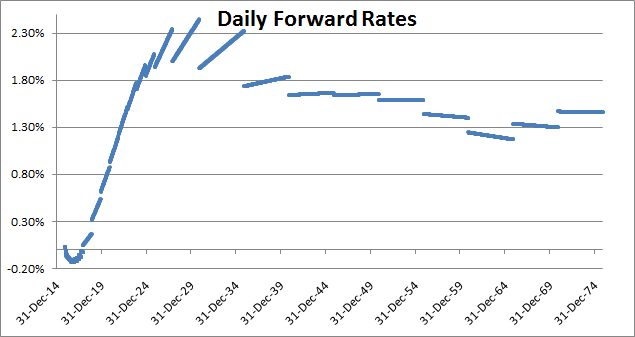
\includegraphics[width=0.7\textwidth]{images/piecewiselinear.png}
        \caption{Piecewise linear interpolation on forward rates on Euribor 6M curve.}
        \label{fig:piecewiselinear}
        \end{figure}
        
        \begin{figure}[!h]
        \centering
        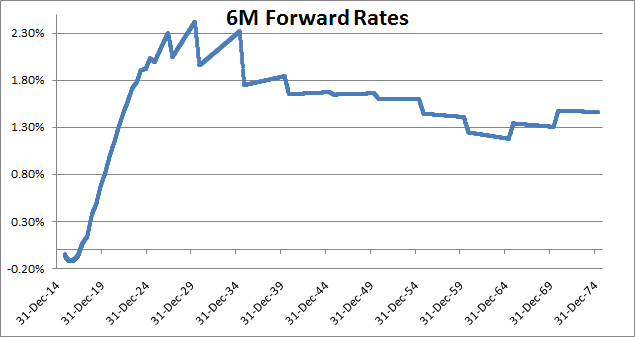
\includegraphics[width=0.7\textwidth]{images/sawtooth.png}
        \caption{Euribor 6M sawtooth curve.}
        \label{fig:sawtooth}
        \end{figure}
        
        Obviously, this is not a good way to interpolate; forward rates are far to be smooth and curve shape is quite improbable.\\
        In the log-discount case, instead, we have the formula:\\
        \\
        $$z(t)t=-\ln P(t)=-\frac{t-t_{i-1}}{t_{i}-t_{i-1}}\ln P(t_{i})-\frac{t_{i}-t}{t_{i}-t_{i-1}}\ln P(t_{i-1})$$\\
        \\
        In this case the output is the so called: "Stepped curve" as visible in Figure \ref{fig:piecewiseflat} and Figure \ref{fig:stepped}. The result is not better than the one obtained with the linear interpolation on zero rates. Nevertheless this method is more popular because that it can be used to describe the first section of overnight-related curves; In fact, market evidence shows that short rates tend to be constant (flat) between particular dates, namely the ones in which there is a European Central Bank monetary policy board meeting. Therefore, the overnight curve case is a particular one in which curve smoothness is a requirement not strictly recommended before the last ECB meeting date published (usually maximum 2 year forward) but returns to be important after it. In this situation using a piecewise flat interpolation or a cubic one for the whole curve might be not accurate in both cases and so we need a merger of both interpolation techniques which leads to the so called: "Mixed interpolation" that will be treated in .....\\
        
        \begin{figure}[!h]
        \centering
        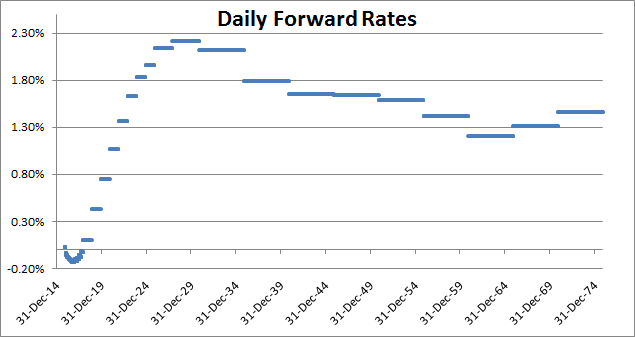
\includegraphics[width=0.7\textwidth]{images/piecewiseflat.png}
        \caption{Piecewise flat forward rates obtained through linear interpolation on log-discounts.}
        \label{fig:piecewiseflat}
        \end{figure}
        
        \newpage
        \begin{figure}[!h]
        \centering
        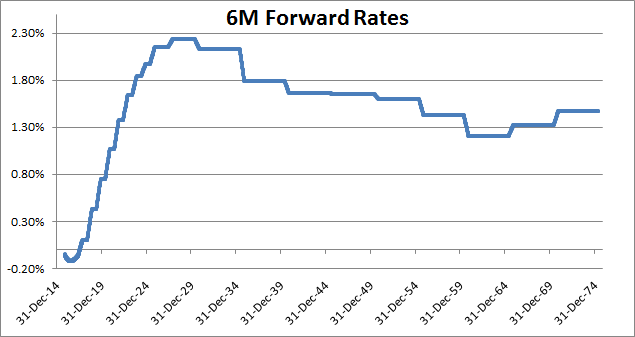
\includegraphics[width=0.7\textwidth]{images/stepped.png}
        \caption{An example of stepped Euribor 6M curve.}
        \label{fig:stepped}
        \end{figure}
        
        \subsection{Constrained Cubic Spline interpolation: The Kruger Scheme} \label{subsection:1.3.3}
        \subsection{Monotonic Cubic Natural Spline interpolation: The Hyman Scheme} \label{subsection:1.3.4}
        
%\blankpagestyle{headings}
%\lipsum[1-2]

%%%CHAPTER2%%%

\chapter{Overnight Curve Definition} \label{chap:2}
    \section{Instrument selection criteria}
        \subsection{Overnight Deposits} \label{subsection:2.1.1}
        \subsection{Overnight Indexed Swap {\it (OIS)}} \label{subsection:2.1.2}
        \subsection{ECB Dated OIS} \label{subsection:2.1.3}
    \section{Calibration choices} \label{section:2.2} 

%\selectlanguage{english}
%\EnableFigTabNames

%%%CHAPTER3%%%

\chapter{Improving Overnight Curve} \label{chap:3}
    \section{Mixed Interpolation}\label{section:3.1}
    \section{Forward Stub for overlapping Instruments} \label{section:3.2}
    This section is devoted to the presentation and solution of a particular ON curve problem due to the manage of the first ECB dated OIS. As already presented in \ref{subsection:2.1.3}, this kind of instruments are forward start OIS that must be included in the curve calibration because of their liquidity. The problem occurs because spot starting OIS maturity dates does not coincide with the settlement date of the first ECB OIS and this leads to a situation in which there are two solutions but either of them produces good results:
    
     \begin{itemize}
         \item{} A possibility is to include all spot starting OIS taking no care of the fact that certainly one of them will have an overlapping maturity date with the forward start ECB OIS. This solution's benefit is that the ON curve will be totally covered because the bootstrap algorithm can manage a sequence of maturities which permits a "pillar-to-pillar" standard bootstrap. Otherwise this choice implies that there will be a short time-frame presenting overlapping instruments as visible in Figure \ref{fig:overlapping}.
         
        \begin{figure}[!h]
        \centering
        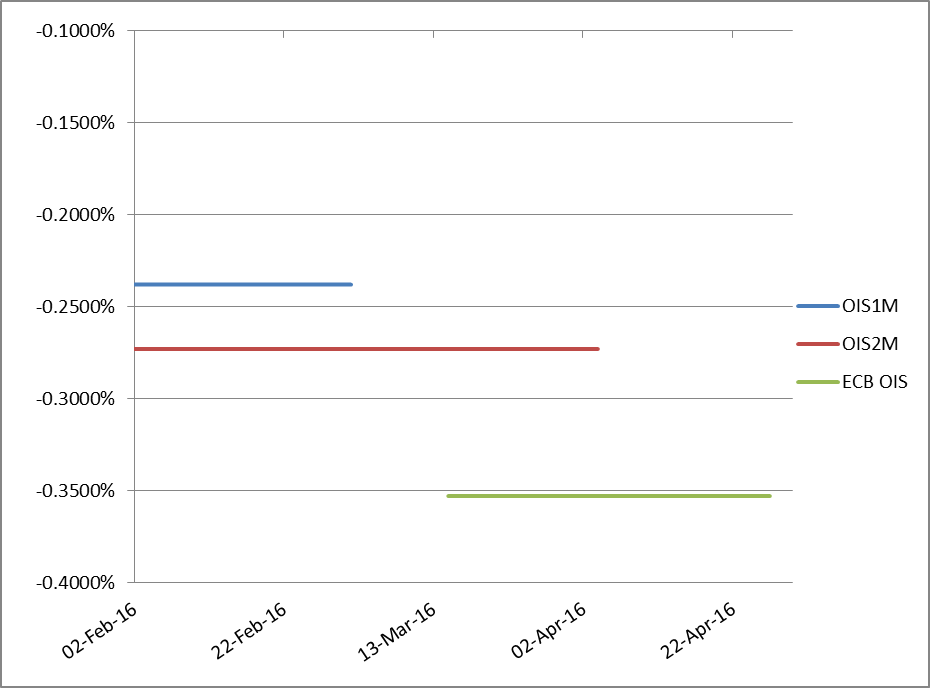
\includegraphics[width=0.6\textwidth]{images/overlapping.png}
        \caption{The overlapping solution using 2 February 2016 values.}
        \label{fig:overlapping}
        \end{figure}
        
        The example shows that OIS with 2-month maturity ({\it 4 April 2016}) overlaps the first ECB OIS with settlement ({\it 16 March 2016}). This 18 days year fraction cause oscillations in the curve's shape and, as a consequence, an impact on not included instruments repricing errors. This errors are also deeply connected to the first section curve's shape; in fact this solution may leads negligible repricing errors only if spot starting OIS and first ECB OIS presents close values (which means that the first curve section tends to be flat). Otherwise, empirical evidence shows that, sometimes, market idiosyncrasies can affect first section curve's shape making it highly downward/upward sloping (as the Figure \ref{fig:overlapping} suggest). In this particular cases also the overlapping solution fails leading to relevant errors as it will be shown in \ref{subsection:3.2.2}.
        
        \item{} Another possible solution may be to exclude from the bootstrap the overlapping OIS (the 2-month maturity one in reference to the preceding example). The benefit of this choice is to avoid overlapping instruments but implies that there will be a not covered curve section, as visible in Figure \ref{fig:exclude}, in which the bootstrap algorithm does not have any information related to the curve shape. The impact of this solution on repricing errors is very bad and so it is not advisable to use it. 
        
        \begin{figure}[!h]
        \centering
        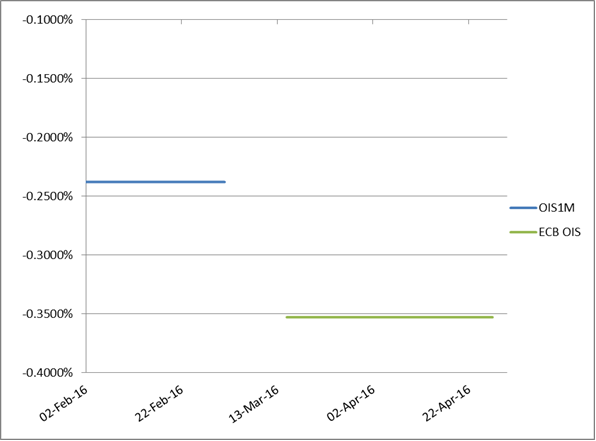
\includegraphics[width=0.6\textwidth]{images/exclude.png}
        \caption{The excluding solution using 2 February 2016 values.}
        \label{fig:exclude}
        \end{figure}
        
        This answers are not satisfactory and seems that there is no solution taking advantage of the only market instruments.\\
        This work's suggestion is to create a forward "Meta-Instrument", from now called {\it Stub}, which implied value can be derived from available market quotes as it will be discussed in next section.
        
        \end{itemize}

        \subsection{Implied value calculation} \label{subsection:3.2.1}
        Let's suppose now to be in the situation described in Figure \ref{fig:exclude} in which there is a not covered curve's section. The Stub quote represents a forward rate which starts from the last not-overlapping instrument's (in the previous example the OIS1M) maturity date and the first ECB Dated settlement date.\\
        
        \begin{figure}[!h]
        \centering
        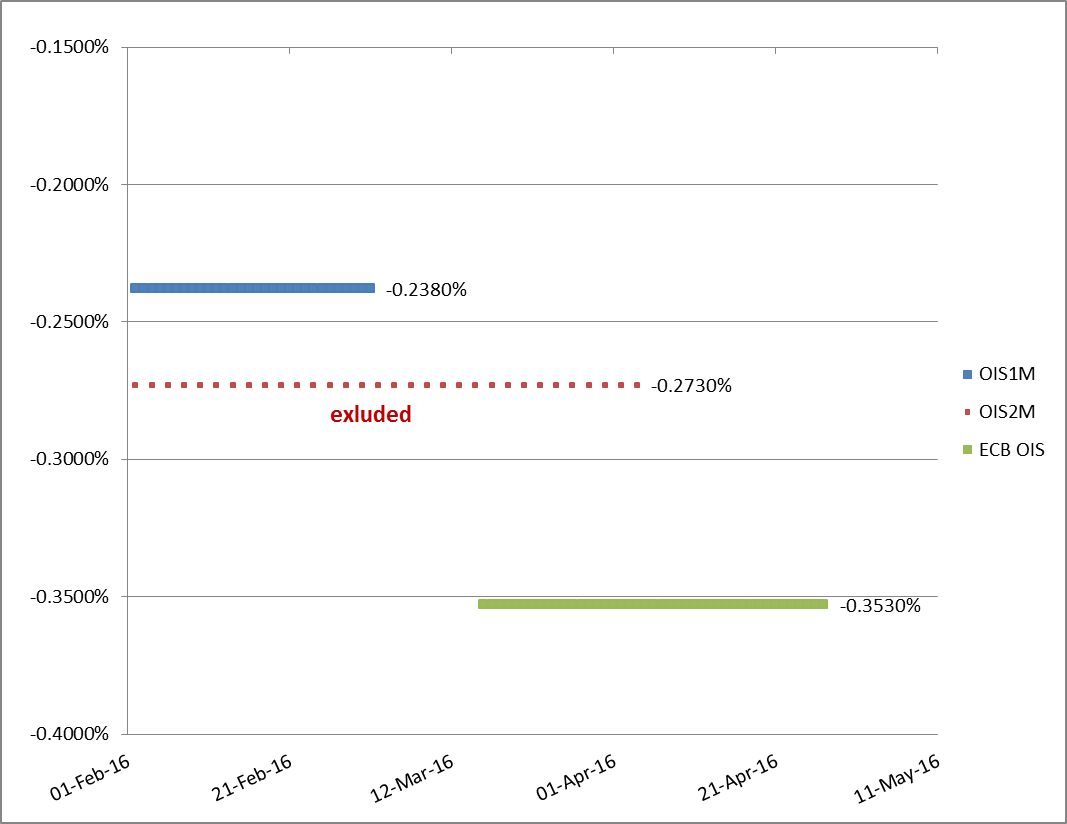
\includegraphics[width=0.6\textwidth]{images/excluded2.png}
        \label{fig:excluded2}
        \end{figure}
        
        This values is implied in the market and can be derived assuming a no-arbitrage condition. In order to not introduce arbitrages, it is necessary to obtain the Stub quote imposing that it must reprice exactly the excluded instrument (OIS2M in above Figure). In order to replicate the OIS2M value the following relationship must hold:
        
        $$e^{\int_{0}^{t\ped{1}} f_{inst}ds} \cdot e^{\int_{t\ped{1}}^{t\ped{2}} f_{inst}ds} \cdot e^{\int_{t\ped{2}}^{t\ped{3}} f_{inst}ds} = e^{\int_{0}^{t\ped{3}} f_{inst}ds}$$
        
        where: 
        $$t\ped{1} = \mbox{Last non-overlapping instrument's maturity in year fraction}$$
        $$t\ped{2} = \mbox{First ECB Dated OIS settlement date  in year fraction}$$
        $$t\ped{3} = \mbox{Overlapping instrument's maturity date in year fraction}$$
        $$f_{inst} = \mbox{Instantaneous forward rate}$$
        
        \begin{figure}[!h]
        \centering
        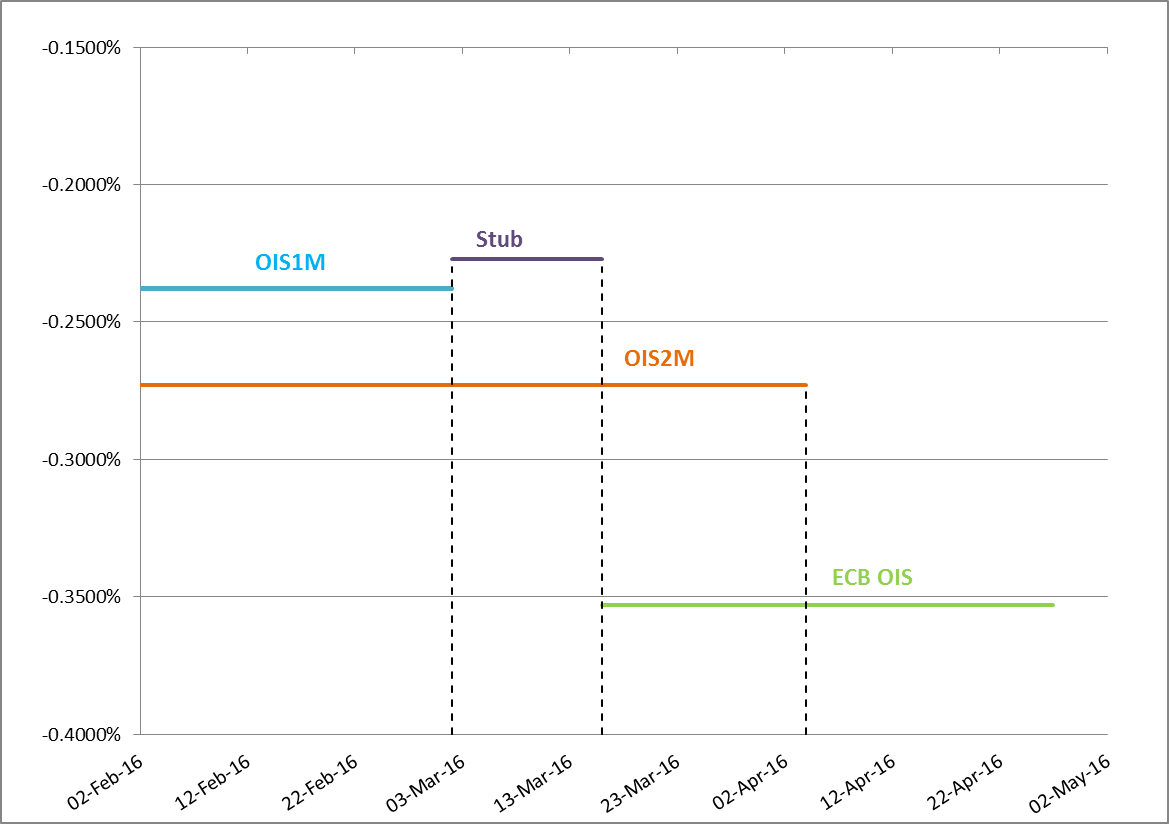
\includegraphics[width=0.6\textwidth]{images/stub.png}
        \caption{The Stub solution using 2 February 2016 values.}
        \label{fig:stub}
        \end{figure}
        
        As visible in Figure \ref{fig:stub}, no-arbitrage condition implies that investing in OIS1M ({\it blue line}), Stub ({\it violet line}) and in ECB OIS till the OIS2M maturity ({\it green line}) must be equal to investing in OIS2M ({\it orange line}). In this situation, the Stub implied value can be easily calculates as:\\
        
        $$ e^{\int_{t\ped{1}}^{t\ped{2}} f_{inst}ds} = \frac{e^{\int_{0}^{t\ped{3}} f_{inst}ds}}{e^{\int_{0}^{t\ped{1}} f_{inst}ds} \cdot e^{\int_{t\ped{2}}^{t\ped{3}} f_{inst}ds}} $$
        \\
        Assuming simple compounding:\\
        
        $$ \mbox{{\it Stub}} = \frac{1+F\ped{0 x t\ped{3}} \cdot \tau\ped{0 x t\ped{3}} }{(1+F\ped{0 x t\ped{1}} \cdot \tau\ped{0 x t\ped{1}}) \cdot (1+F\ped{t\ped{2} x t\ped{3}} \cdot \tau\ped{t\ped{2} x t\ped{3}})} $$\\
        \\
        Introducing in the calibration this forward Stub improve consistently the ON curve goodness avoiding unwanted distortion and oscillation as will be shown in next session.
        Otherwise, this solution can be implemented only if the bootstrap algorithm uses a log-linear interpolation for the first curve's section. Interpolating log-linearly the ON curve becomes piecewise constant, as seen in \ref{subsection:1.3.1}, and this assumption permits to derive the $e^{\int_{t\ped{2}}^{t\ped{3}} f_{inst}ds}$ value that must be equal to ECB OIS market quote. The good news is that, as seen in \ref{section:3.1}, the best practise to interpolate the ON curve is by means of a mixed interpolation, which interpolates log-linearly the first 2 years curve's section. \\
        
        \subsection{Impact on Curve and Repricing Errors} \label{subsection:3.2.2}
        In the previous section it has been presented a particular ON curve problem and 3 possible ways to solve it. Let's start from the worst one, namely the solution in which the overlapping instrument is excluded leaving a non-covered curve's section. With this 
        approach the curve obtained is represented in the underlying figure:\\
        
        \begin{figure}[!h]
        \centering
        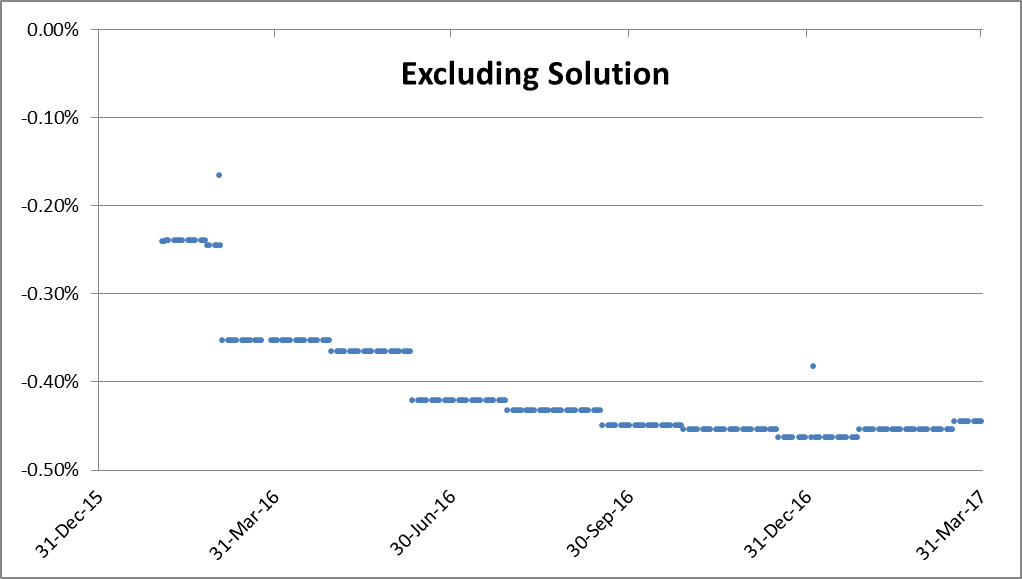
\includegraphics[width=0.7\textwidth]{images/excludingcurve.png}
        \caption{ON Curve excluding overlapping instrument (Evaluation date 2 February 2016).}
        \label{fig:excludingcurve}
        \end{figure}
        
        This solution's big problem is that the bootstrap algorithm extrapolate backward from ECB Dated market quote the non-covered curve's part leading to high distortions especially when preceding instrument and ECB OIS quotes are distant.\\
        A better solution can be including all spot starting OIS even if one of them will certainly be overlapping. This approach is described in next figure:\\
        
        \begin{figure}[!h]
        \centering
        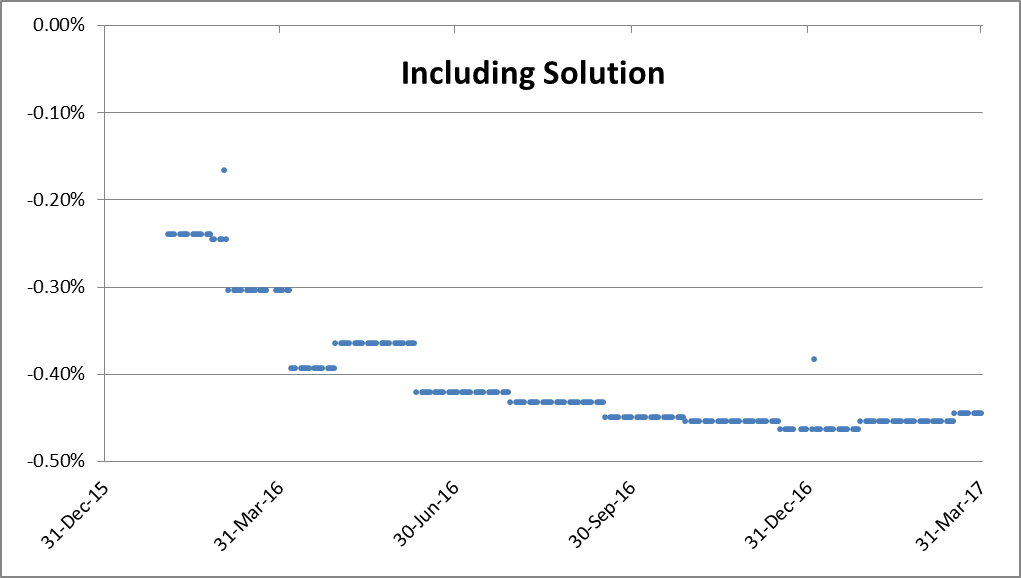
\includegraphics[width=0.7\textwidth]{images/includingcurve.png}
        \caption{ON Curve including overlapping instrument (Evaluation date 2 February 2016).}
        \label{fig:includingcurve}
        \end{figure}
        
        \newpage
        As it will be shown soon this solution produces distortions due to the fact that the calibration must introduce strange oscillations in order to reprice the overlapping instrument. In fact, the Figure \ref{fig:includingcurve}, shows how the curve is pushed down till $-0.40\%$ and then turns back to the ECB OIS level. It is quite obvious that this strange curve's behaviour is not due to market quotes but to calibration's discrepancy resulting from the overlapping section.\\
        Finally, let's present the forward Stub solution in the underlying figure:\\
        
        \begin{figure}[!h]
        \centering
        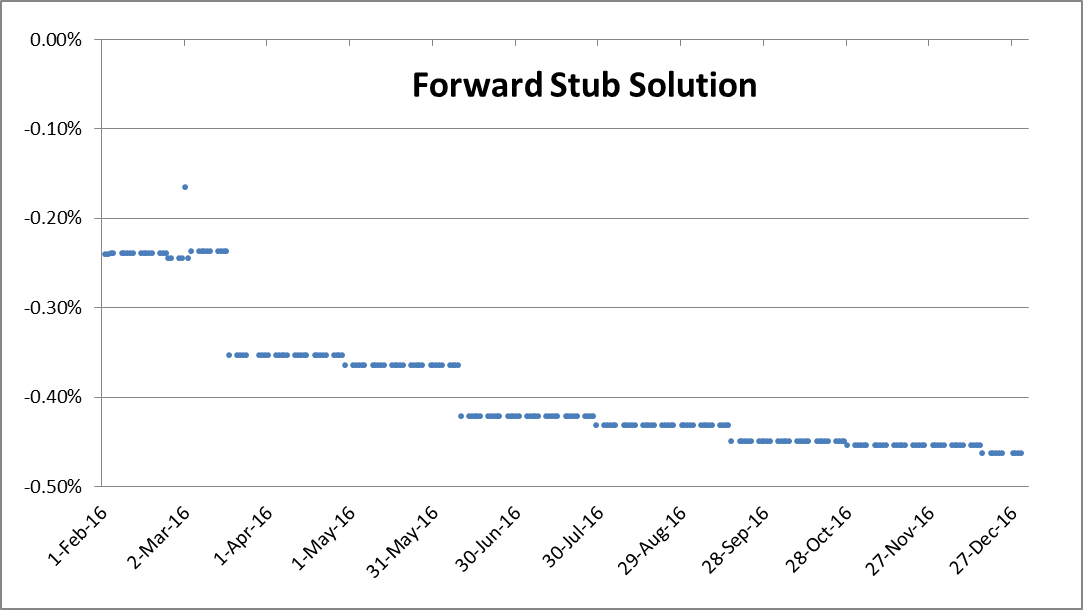
\includegraphics[width=0.7\textwidth]{images/stubcurve.png}
        \caption{ON Curve including forward Stub (Evaluation date 2 February 2016).}
        \label{fig:stubcurve}
        \end{figure}
        
        \newpage
        As visible, there are no wide oscillation in the curve's shape and the repricing errors analysis, represented in Figure,  shows that this approach is the one which minimize all out-of-curve instruments, ensuring also the perfect reprice of the overlapping instrument excluded.
        
        \begin{figure}[!h]
        \centering
        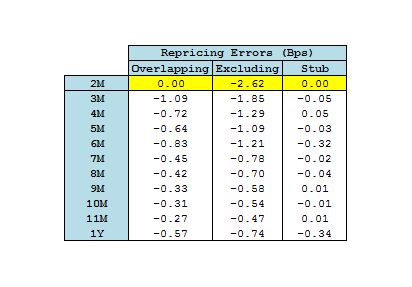
\includegraphics[width=0.7\textwidth]{images/errors.png}
        \caption{Repricing errors summary for all possible solutions.}
        \label{fig:errors}
        \end{figure}
        
    \section{Jumps Inclusion} \label{section:3.3}
        \subsection{The EUR market case: Positive Jumps} \label{subsection:3.3.1}
        \subsection{The GBP and USD market case: Negative Jumps} \label{subsection:3.3.2}
    \section{Fed Funds Arithmetic Average Coupon OIS} \label{section:3.4}
        \subsection{Valuation and Bootstrapping} \label{subsection:3.4.1}
        \subsection{Hull \& White Model calibration for Convexity Adjustment estimation} \label{subsection:3.4.2} 

%%%CONCLUSION%%%

\chapter*{Conclusion} \label{chap:Concl}
\markboth{\MakeUppercase{Conclusion}}{}
\addcontentsline{toc}{chapter}{Conclusion}

%%%APPENDICES%%%

\newpage
\appendix

\begin{appendices}
  \renewcommand\thetable{\thesection\arabic{table}}
  \renewcommand\thefigure{\thesection\arabic{figure}}
\chapter{Interest Rate Conventions} \label{app:Conv}
With the next two appendices i want to go a step back. The main goal of this work is outline the most important steps related to curve calibration techniques, with particular attention to the overnight one, and this involve a deep understanding of interest rate calculation and conventions but also of the whole set of financial instruments involved in the bootstrap procedure. 
The one first is devoted to introduce some basic and fundamental interest rate rule in order to fix the idea that there are different ways to obtain an interest rate that are strictly connected to the compounding rule chosen, to the way in which time is calculated and to the type of interest we want to derive.
    \section{Capitalization and Discount Factors}
    We are all familiar with the concept that cash availability it's a privilege we don't want to give up for free. Of course, everyone who has an amount of money want to be compensated if he decides to lend it and this is the reason why negative interests rates were unthinkable. however, today's index fixings are deeply below zero due to very expansive Central Bank's monetary policy and, in this scenario, a future amount of money worth less than the same amount of money owned today. Aside from negative rates issue, what we need is answer to the questions:
    \begin{description}
        \item{-} What is the future value of a today's amount of money?
        \item{-} What is the present value of a future cash flow?
    \end{description}
    To answer we have to introduce Capitalization and Discount Factors.
    The capitalization factor: $h(R,(t_2-t_1))$ measures the future value, after the year fraction $(t_2-t_1)$ (from now $\tau$) of a unit of currency owned today; instead, the discount factor: $\frac{1}{h(R,\tau)}$ measures the present value of a unit of currency paid after the year fraction $\tau$. This premise is necessary to introduce an important notion that has been true for a long time but not anymore, namely that capitalization factors are an increasing function of time and, consequently, their inverse, the discount factors, are a decreasing function of time.\\
    Naming:\\
    $$D(t) \mbox{ the discount factor in }  t, \mbox{ and:}$$ 
    $$C(t) = \frac{1}{D(t)} \mbox{ the capitalization faction in } t$$\\
    we have that, {\bfseries assuming positive interest rates}:\\
    $$D(t) < 1 \mbox{ for any } t > 0$$
    $$D(t_1) > D(t_2) \mbox{ if } t_1<t_2\mbox{ and:}$$
    $$C(t) > 1 \mbox{ for any } t > 0$$
    $$C(t_1) < C(t_2) \mbox{ if } t_1<t_2\mbox{ and:}$$\\
    As we will see, define the function $h(R,\tau)$ isn't so easy as it seems because the capitalization formula can be measured in different ways.
    Changing parameters has a strong impact on capitalization/discount factors; therefore, it's fundamental to take confidence with all kinds of parametrization starting from compounding rules.
    \section{Compounding Rules}
    For compounding rule we mean a method to calculate the future value of an amount of money. The easier way to describe $h(R,(t_2-t_1))$ function is to use the {\itshape simple compounding scheme}.
        \subsection{Simple Compounding}
        This scheme implies that: $$ I = N*R*\tau$$ $$N+I=N*(1+R*\tau)$$ where $I$ is the interest amount in $t_2$ and $N$ is the notional at the beginning of the accrual period ($t_1$). Accordingly, the Capitalization Factor in simple compounding is: 
        $$C(t) = h(R,\tau) = (1+R*\tau)$$\\
        and the Discount Factor is: 
        $$D(t) = \frac{1}{h(R,\tau)} = \frac{1}{(1+R*\tau)}$$
        Therefore, the capital grows linearly during time because interest amounts are not capitalized to produce other interests.
        \subsection{Compounded Interest Rate}
        In this scheme interests are compounded $m$ times per year for $\tau$ years at rate R. So, investing a notional N produce at the end of the accrual period:
        $$N*\left(1+\frac{R}{m}\right)^{m\tau}$$   
        The compounded Capitalization and Discount Factors, therefore, are:
        $$C(t) = h(R,\tau) = \left(1+\frac{R}{m}\right)^{m\tau}$$ 
        $$D(t) = \frac{1}{h(R,\tau)} = \left(1+\frac{R}{m}\right)^{-m\tau}$$
        Using the compounded scheme means that, every $m$ times the interest is compounded, the capital accrued become the new initial capital and this means that interests are producing other interests. 
        \subsection{Continuous Compounding}
        This compounding rule can be view as a particular case of the preceding one in which we imagine to compound more and more frequently simply taking the limit of $m$ tending to infinity. Expressing this concept in formulas the continuously compounded interest rate is given by:
        $$\lim_{m\rightarrow+\infty} N*\left(1+\frac{R}{m}\right)^{m\tau} = N*e^{R\tau}$$
        Hence, the Capitalization and Discount factors in continuous compounding are:
        $$C(t) = h(R,\tau) = e^{R\tau}$$ 
        $$D(t) = e^{-R\tau}$$
        A good approximation of the continuous interest is to do the daily compounded interest rate. Assuming a year composed by 365 days we have that:
        $$e^{R\tau} \approx \left(1+\frac{R}{365}\right)^{-365\tau}$$
    \section{Day-Count Conventions}
    After having specified how the interest can be compounded, we have to describe how we can measure the year fraction $\tau = (t_2-t_1)$. For a easier computation, market participants use different kind of conventions called {\itshape Day Counter}; let's describe the most popular:
    \begin{itemize}
    \item \textit{Actual/360} : where \textit{Actual} is the number of days between the two dates.
    $$Actual/360 = \frac{d_2-d_1}{360}$$
    \item \textit{Actual/365 (fixed)}: where \textit{Actual} is defined as before and 365 is used even in a leap year.
    $$Actual/365 (fixed) = \frac{d_2-d_1}{365}$$
    \item \textit{30/360}: where the numerator is obtained as:
    $$360 \cdot(Y_2-Y_1)+30*(M_2-M_1)+(d_2-d_1)$$ with $Y = \mbox{year}$, $M = \mbox{month}$, $d = \mbox{day}$.\\
    The date adjustment rules are the following:
    \begin{itemize}
    \item if $d_1$ is $31$ then change $d_1$ to 30;
    \item if $d_2$ is $31$ then change $d_2$ to 30. 
    \\
    \end{itemize}
    $$30/360 = \frac{360*(Y_2-Y_1)+30*(M_2-M_1)+(d_2-d_1)}{360}$$
    \\
    \end{itemize}
    It's evident that the day counter choice affects directly the measure of the accrual period, and so, the    interest accumulated.
    \section{Calendar}
    Banks and stock exchange are not open every day for business, so we need to define a set of dates in which two legal entities agree to exchange cash flows, the so called business calendar. We can find different calendar depending on which area we are dealing with. For EURO currency, for example, we have TARGET (Trans-European Automated Real-time Gross settlement Express Transfer) calendar, for GBP (Great Britain Pound) we have London Stock Exchange Calendar with a different set of holidays and so on.
    \section{Business Day Conventions}
    which determines how non-business days have to be treated. Imagine, for example, that a ZCB (\textit{Zero Coupon Bond} payment date falls on a holiday; the counterparts need a pre-decided rule which stabilizes if the payment have to be anticipated or postponed. This types of conventions have properly this aim and the most widely used are:
    \\
    \begin{itemize}
    \item Following (defined by the International Swaps and Derivatives Association: ISDA): choose the first business day after the given holiday;
    \item Modified Following (ISDA): choose the first business day after the given holiday, unless it belongs to a different month; in that case choose the first business day before the given holiday;
    \item Preceding (ISDA): choose the first business day before the given holiday;
    \item Modified Preceding (ISDA): choose the first business day before the given holiday, unless it belongs to a different month; in that case choose the first business day after the given holiday;
    \item Unadjusted: use the given date even if it is an holiday.
    \end{itemize}
    \section{Evaluation and Settlement Date}
    We need to do a distinction between the \textit{Settlement Date}, namely the date in which an investment starts to earn interests, and \textit{Evaluation Date} (or \textit{Fixing Date}), the date in which contracts are traded, because frequently they aren't the same.\\
    For example, in EURO Market the \textit{Settlement Date} is 2 business days after the \textit{Evaluation Date}; so if today a trader make a 1 month investment at rate $R$, the accrual period doesn't starts today but 2 business days after; consequently, the maturity date will be 1 month after the \textit{Settlement Date} and not the \textit{Evaluation Date}.
    \section{Types of Interest Rates}
    A final and crucial description must be dedicated to each type $R$ we can use in the $h(R,\tau)$ function. in this context we have to define 3 different classes of rates, namely:
    \begin{itemize}
    \item{\bfseries Zero Rates (or Spot Rates)}: it's the rate of interest earned on an investment that starts accruing interests from today $(= \mbox{spot date})$ and provides a unique payoff only at maturity date (no intermediate coupons).
    \item{\bfseries Forward Rates}: it's the rate of interest earned on an investment that starts accruing at a future date $(> \mbox{spot date})$ and provides a unique payoff. A forward rate represents the most probable expectation for the future fixing of the present zero rate. Before the beginning of the Multi-Curve World, moving on a single standard curve leads to a situation that it was always possible to calculate the implied forward rate starting from 2 zero rates. To fix this concept let's make an example:\\
    Suppose that today's interest rate term structure shows that a 3 months deposit market value is $r\ped{0 \times 3}$ and a 6 months deposit market value is $r\ped{0 \times 6}$. In the old Single-Curve World we were always able to calculate the (3X6) F.R.A. implied quote $f\ped{3 \times 6}$ (that represents the interest rate payed by an investment which starts from a 3  months forward date and ends 3 months after). Taking advantage of no arbitrage theory this relation must always old: 
    $$1 \cdot e^{r\ped{0 \times 6} \cdot t\ped{2}} = 1 \cdot e^{r\ped{0 \times 3} \cdot t\ped{1}} \cdot e^{F\ped{1 \times 2} \cdot (t\ped{2} - t\ped{1})}$$
    $$e^{r\ped{0 \times 6} \cdot t\ped{2}} = e^{r\ped{0 \times 3} \cdot t\ped{1} + F\ped{1 \times 2} \cdot (t\ped{2} - t\ped{1})}$$
    $$r\ped{0 \times 6} \cdot t\ped{2} = r\ped{0 \times 3} \cdot t\ped{1} + F\ped{1 \times 2} \cdot (t\ped{2} - t\ped{1})$$
    $$F\ped{3 \times 6} = \frac{r\ped{0 \times 6} \cdot t\ped{2} - r\ped{0 \times 3} \cdot t\ped{1}}{(t\ped{2} - t\ped{1})}$$C
    \\
    Applying the same formula for discount factors we derive that:
    $$F\ped{3 \times 6} = \frac{1}{(t\ped{2} - t\ped{1})} \cdot \ln\left(\frac{D\ped{0 \times 3}}{D\ped{0 \times 6}}\right)$$
    \\
    \item{\bfseries Instantaneous Forward Rates}: Let's now assume that we want to compute a forward rate starting from $t$ and for a very short time interval $dt$. Using previous equation we get that:
    $$f\ped{t \times (t+dt)} = \frac{1}{(dt)} \cdot \ln\left(\frac{D\ped{t}}{D\ped{t+dt}}\right)$$
    Taking the limit of $dt$ tending to $0$ we get the so called Instantaneous Forward Rate $f\ped{t \times (t+dt)}$, where $dt$ is an infinitesimal time fraction. It is also possible to define a relationship between zero rates, forward rates and instantaneous forward rates:
    $$F_{t\ped{1},t\ped{2}} = \frac{1}{(t\ped{2} - t\ped{1})} (e^{\int_{t\ped{1}}^{t\ped{2}} f_{inst}ds}-1)$$
    $$r_{0 \times t} = \frac{1}{t} \int_{0}^{t} f_{inst}ds$$
    It is observable that a zero rate is the average of $f_{inst}$ over the interval $[0,t]$ and, consequently, a forward rate is the average of  $f_{inst}$ over the interval $[t\ped{1},t\ped{2}]$. This leads to the following relationship:
    $$D(0,t) = e^{-(r\ped{0 \times t} \cdot t)} = e^{- \int_{0}^{t} f_{inst}ds}$$
    \end{itemize}

\end{appendices}

%%%BIBLIOGRAPHY%%%

\begin{thebibliography}{9}
\end{thebibliography}

\end{document}